\chapter{The nuclear model with explicit mesons :D}\label{Decsofmodel}

We consider a nuclear model where the nucleus is held together by emitting and absorbing mesons, and the mesons are treated explicitly \cite[]{Mesons}. We are considering the regime of low-energy nuclear physics and this model is different from conventional interaction models in several ways. Firstly, the nucleons interact by emitting and absorbing mesons and not via a phenomenological potential. Conceptually this is similar to the one-boson-exchange model. Secondly, the number of parameters is greatly reduced. Regardless of the meson type, the number of parameters is two; the range and the strength of the meson-nucleon coupling are denoted $b$ and $S$ respectively. In the case of the pion, the central force, tensor force and the three-body force are all concealed within these two parameters. This model should be able to reproduce phenomena within the realm of low-energy nuclear physics such as the deuteron, nucleon-nucleon scattering, pion-nucleon scattering and pion photoproduction. The low energy regime also enables the use of the Schrödinger equation to describe the equations of motion. The model must be constructed in a way such that usual quantum numbers are conserved; this means conservation of isospin, angular momentum and parity. 

\section{Nuclear interacting model with explicit pions }\label{sec:model}

In the following, we focus on the nuclear model with explicit pions. The pion is the lightest of the strongly interacting particles with a mass of about $15\%$ of the nucleon mass. This yields a large Compton wavelength of $1.4$ fm which means the longest contribution to nucleon-nucleon interactions. Furthermore, the pion is a significant component of the nuclear wave function where the pion dominates meson exchange corrections to different nuclear properties. In general, the bare nucleon is surrounded by several virtual pions. 
They are virtual in the same sense that the positron-electron pair are virtual in pair creation from a photon. It is important to stress the fact that these are virtual since they can have properties possible for true particles. The multi-component wave function of the nucleon can be written as
\begin{marginfigure}
	\centering
	

\tikzset{every picture/.style={line width=0.75pt}} %set default line width to 0.75pt        

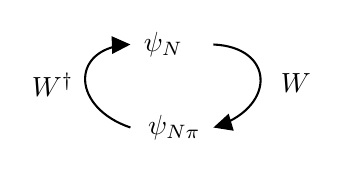
\begin{tikzpicture}[x=0.75pt,y=0.75pt,yscale=-1,xscale=1]
	%uncomment if require: \path (0,300); %set diagram left start at 0, and has height of 300
	
	%Curve Lines [id:da45911359937309637] 
	\draw    (280,60) .. controls (309.18,61.28) and (310.43,89.17) .. (282.66,99.13) ;
	\draw [shift={(280,100)}, rotate = 343.41] [fill={rgb, 255:red, 0; green, 0; blue, 0 }  ][line width=0.08]  [draw opacity=0] (8.93,-4.29) -- (0,0) -- (8.93,4.29) -- cycle    ;
	%Curve Lines [id:da6231994153364976] 
	\draw    (240,100) .. controls (211.9,90.47) and (210.92,62.94) .. (237.05,60.2) ;
	\draw [shift={(240,60)}, rotate = 178.19] [fill={rgb, 255:red, 0; green, 0; blue, 0 }  ][line width=0.08]  [draw opacity=0] (8.93,-4.29) -- (0,0) -- (8.93,4.29) -- cycle    ;
	
	% Text Node
	\draw (245,52.4) node [anchor=north west][inner sep=0.75pt]    {$\psi _{N}$};
	% Text Node
	\draw (247,92.4) node [anchor=north west][inner sep=0.75pt]    {$\psi _{N\pi }$};
	% Text Node
	\draw (191,72.4) node [anchor=north west][inner sep=0.75pt]    {$W^{\dagger }$};
	% Text Node
	\draw (311,72.4) node [anchor=north west][inner sep=0.75pt]    {$W$};
	
	
\end{tikzpicture}
	\caption{Illustration of the pion-nucleon operator, $W$}
	\label{fig:superposition}
\end{marginfigure}

\begin{equation} \label{superposition}
	\Psi_N = \mqty[\psi_{N} \\
	\psi_{N\pi} \\
	\psi_{N\pi\pi}\\
	\vdots],
\end{equation}
where $\psi_{N}$ is the bare nucleon and the other wave functions are dressed by an arbitrary number of pions indicated by the subscripts. Assuming the nuclear interaction conserved isospin, angular momentum and parity we can construct the following operator for the pion-nucleon operator
\begin{align} \label{W}
	W & \equiv (\vec{\tau\cdot\vec{\pi}})(\vec{\sigma}\cdot\vec{r})f(r) \\
	W^\dagger & \equiv  \int_V \text{d}^3 r \, (\vec{\tau\cdot\vec{\pi}})^\dagger (\vec{\sigma}\cdot\vec{r})^\dagger f(r),
\end{align}
where $\vec{\tau}$ is the isovector of Pauli matrices acting on the nucleon in isospin space and $\vec{\sigma}$ is the same but for spin space and $\vec{r}$ is the relative coordinate distance between the nucleon and the pion. These operators ensure the conservation of isospin, angular momentum and parity. The isovector of pions is denoted $\vec{\pi}$ and can be combined with $\vec{\tau}$ can be represented as a traceless 2-by-2 hermitian matrix given by
\begin{equation} \label{isocoeff}
	\vec{\tau}\cdot \vec{\pi} = \tau_0  \pi_0+ \sqrt{2} \tau_{-}\pi^ +\sqrt{2}\tau_{+} \pi^{-} = \mqty[\pi^0 & \sqrt{2}\pi^- \\
	\sqrt{2}\pi^+ & -\pi^0],
\end{equation}
where the isospin coefficients will be important later when we discuss different photoproduction processes. Similarly, by expanding the matrices in spin space and using the spherical tensor operator we get the following matrix in terms of the spherical harmonics
\begin{equation}\label{spinmatrix}
	\vec{\sigma}\cdot \vec{r} = \sqrt{\frac{4\pi}{3}} r \mqty[Y_{1}^0 & \sqrt{2}Y_1^{-1} \\ \sqrt{2}Y_1^1 & Y_1^0],
\end{equation}
where similar to in isospin space, the off-diagonals include a factor $\sqrt{2}$.  
\begin{marginfigure}
	\centering
	

\tikzset{every picture/.style={line width=0.75pt}} %set default line width to 0.75pt        

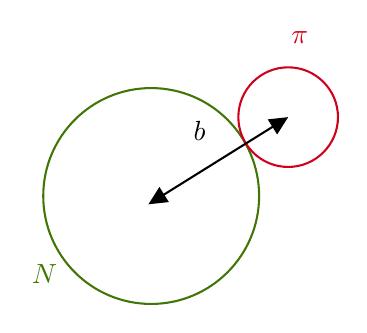
\begin{tikzpicture}[x=0.75pt,y=0.75pt,yscale=-1,xscale=1]
%uncomment if require: \path (0,300); %set diagram left start at 0, and has height of 300

%Shape: Circle [id:dp5217046923283729] 
\draw  [color={rgb, 255:red, 65; green, 117; blue, 5 }  ,draw opacity=1 ] (177,163) .. controls (177,134.28) and (200.28,111) .. (229,111) .. controls (257.72,111) and (281,134.28) .. (281,163) .. controls (281,191.72) and (257.72,215) .. (229,215) .. controls (200.28,215) and (177,191.72) .. (177,163) -- cycle ;
%Shape: Circle [id:dp22288734190325] 
\draw  [color={rgb, 255:red, 208; green, 2; blue, 27 }  ,draw opacity=1 ] (271,125) .. controls (271,111.75) and (281.75,101) .. (295,101) .. controls (308.25,101) and (319,111.75) .. (319,125) .. controls (319,138.25) and (308.25,149) .. (295,149) .. controls (281.75,149) and (271,138.25) .. (271,125) -- cycle ;
%Straight Lines [id:da9107173582949104] 
\draw    (230.21,165.41) -- (292.45,126.59) ;
\draw [shift={(295,125)}, rotate = 148.05] [fill={rgb, 255:red, 0; green, 0; blue, 0 }  ][line width=0.08]  [draw opacity=0] (8.93,-4.29) -- (0,0) -- (8.93,4.29) -- cycle    ;
\draw [shift={(227.67,167)}, rotate = 328.05] [fill={rgb, 255:red, 0; green, 0; blue, 0 }  ][line width=0.08]  [draw opacity=0] (8.93,-4.29) -- (0,0) -- (8.93,4.29) -- cycle    ;

% Text Node
\draw (170,194.4) node [anchor=north west][inner sep=0.75pt]  [color={rgb, 255:red, 65; green, 117; blue, 5 }  ,opacity=1 ]  {$N$};
% Text Node
\draw (295,82.4) node [anchor=north west][inner sep=0.75pt]  [color={rgb, 255:red, 208; green, 2; blue, 27 }  ,opacity=1 ]  {$\pi$};
% Text Node
\draw (248,125.4) node [anchor=north west][inner sep=0.75pt]  [color={rgb, 255:red, 0; green, 0; blue, 0 }  ,opacity=1 ]  {$b$};


\end{tikzpicture}
	\caption{Schematic figure of the system to describe the form factor, \eqref{formfactoreq}. The pion is assumed to sit on the surface.}
	\label{formfactor}
\end{marginfigure}
There is also a phenomenological, short-range form factor $f(r)$ given by
\begin{equation}\label{formfactoreq}
	f(r) = \frac{S}{b} \text{e}^{-r^2/b^2},
\end{equation}
where $S$ and $b$ are the pion-nucleon coupling strength and range respectively--these are illustrated in figure \ref{formfactor}. The action of annihilating a pion must include the integral over coordinate space to remove the coordinate. We now have everything we need to construct a general Hamiltonian for the multi-component wave function of the nucleon in \eqref{superposition}
\begin{equation} \label{multihamiltonian}
	H = \mqty[K_N & W^\dagger & 0 &\ldots \\
	W & K_N+K_\pi+m_\pi c^2+V_C & W^\dagger & \ldots \\
	0 & W & K_N+K_{\pi(1)}+K_{\pi(2)}+2m_\pi c^2 +V_C & \ldots \\
	\vdots & \vdots & \vdots &\ddots ],
\end{equation}
where the kinetic operators are given by
\begin{align} \label{multiN}
	K_N &= \frac{-\hbar^2}{2 m_N c^2} \frac{\partial}{\partial \vec{R}^2} \\
	K_\pi &= \frac{-\hbar^2}{2 m_\pi c^2} \frac{\partial}{\partial \vec{r}^2}.
\end{align} 
Note the different derivatives--here $\vec{R}$ is the center-of-mass coordinate and $\vec{r}$ is the relative coordinate. The subscripts on the kinetic operators in \eqref{multihamiltonian} represent the order in which the pions are created. Should there be charged particles involved one must include a Coulomb interaction denoted by $V_C$. From \eqref{superposition} and \eqref{multihamiltonian} we can construct the general Schrödinger equation
\begin{equation} \label{MultiSE}
	H \Psi_N = E \Psi_N,
\end{equation}
where the ground state is the bare nucleon surrounded by virtual pions. The ground state energy in the rest frame of the nucleon gives the mass of the physical nucleon. Within the framework of this model, one can generate a physical pion by supplying enough energy such that the pion is no longer virtual. The pion is trapped behind a potential barrier of height $m_\pi c^2 = 140$ MeV and cannot leave unless this or more energy is supplied to the system.  
\section{Dressing of the nucleon in the one pion approximation}
We now consider the scenario where a photon interacts with the nucleon-pion systems and generates a physical pion. This means the energy is higher than the potential barrier also when taking recoil effects into account. This also hints how a pion photoproduction process would emerge naturally as a disintegration process in this nuclear model. To generate more pions the photon energy would have to be increased by the same amount. This also means one could assume the first pion is responsible for the largest contribution to the nucleon dressing.  This will be referred to as the one pion approximation.  As a proof-of-concept we constrain ourselves to the one pion approximation and adding more pions should in principle be straight forward extension of the following calculations.


Returning to \eqref{superposition} and enforcing the one pion approximation yields
\begin{equation} \label{2wavefunc}
	\Psi = \mqty[\psi_{N}(\vec{R})\\
		\psi_{N\pi}(\vec{r})].
\end{equation}
The Hamiltonian which acts on the two-component wave function in \eqref{2wavefunc} is given by\footnote{Strictly speaking one should use a three-component wave function to account for the mass difference between $\pi^0$ and $\pi^\pm$. This is done in appendix \ref{ThreeComponentWavefunction}.}
\begin{equation}
	H  =  \mqty[K_N & W^\dagger \\ W & K_N+K_\pi+m_\pi c^2],
\end{equation}
\begin{equation}\label{pnpi}
    \psi_p = p\uparrow\frac{1}{\sqrt{V}}, \quad \psi_{N\pi}=(\vec{\tau\cdot\vec{\pi}})(\vec{\sigma}\cdot\vec{r})\phi(r)p\uparrow\frac{1}{\sqrt{V}},
\end{equation}
where $V$ is the volume, $\vec{\tau}$ is combination of the matrices $\tau_{1,2,3}$ into a matrix vector--completely analogous to the vector $\vec{\sigma}$ of spin Pauli matrices. Also, we have chosen the proton as isospin up state in the nucleon
\begin{equation}
    \ket{p} = \mqty[1 \\ 0].
\end{equation}
From \eqref{pnpi}
\begin{equation} \label{wavefunc}
    \Psi = \mqty[\psi_p \\ \psi_{N\pi}],
\end{equation}
To construct a Hamiltonian we define two operators corresponding to creation and annihilation of the meson. We define the operator as 
\begin{marginfigure}
\centering
\tikzset{every picture/.style={line width=0.75pt}} %set default line width to 0.75pt        

\begin{tikzpicture}[x=0.75pt,y=0.75pt,yscale=-0.75,xscale=0.75]
%uncomment if require: \path (0,414); %set diagram left start at 0, and has height of 414

%Straight Lines [id:da3197661690361302] 
\draw    (150,60) -- (337.33,113.33) ;
%Straight Lines [id:da09724210631479624] 
\draw    (218.97,82.82) -- (180,190) ;
\draw [shift={(220,80)}, rotate = 109.98] [fill={rgb, 255:red, 0; green, 0; blue, 0 }  ][line width=0.08]  [draw opacity=0] (8.93,-4.29) -- (0,0) -- (8.93,4.29) -- cycle    ;

% Text Node
\draw (137,42.4) node [anchor=north west][inner sep=0.75pt]    {$N$};
% Text Node
\draw (346,112.4) node [anchor=north west][inner sep=0.75pt]    {$\pi $};
% Text Node
\draw (171,142.4) node [anchor=north west][inner sep=0.75pt]    {$\vec{R}$};
% Text Node
\draw (267,70.4) node [anchor=north west][inner sep=0.75pt]    {$\vec{r}$};
\end{tikzpicture}
\caption{Absolute and relative distance.}
\label{relativecoordinate}
\end{marginfigure}
\begin{equation} \label{W}
    W \equiv (\vec{\tau\cdot\vec{\pi}})(\vec{\sigma}\cdot\vec{r})f(r),
\end{equation}
where $f(r)$ is some form factor given by
where $S\simeq 10 \, \text{MeV}$  and $b\simeq 1 \, \text{fm}$. This is illustrated in figure \ref{formfactor}. Note that \eqref{formfactoreq} must have units of energy per length such that \eqref{W} has units of energy. 

From \eqref{W} we can construct the Hamiltonian of the system
\begin{equation}
    H \doteq \mqty[K_{\vec{R}} & W^\dagger \\ W & K_{\vec{R}}+K_{\vec{r}}+m_\pi c^2],
\end{equation}
where $K_i$ represents the kinetic term of particle $i$. Also, $R$ represents the absolute distance and $r$ is the relative distance as illustrated in figure \ref{relativecoordinate}. Plugging this into the Schrödinger equation yields 
\begin{equation}\label{SE}
    \mqty[K_{\vec{p}} & W^\dagger \\ W & K_{\vec{R}}+K_{\vec{r}}+m_\pi c^2]\mqty[\psi_p \\ \psi_{N\pi}] = E \mqty[\psi_p \\ \psi_{N\pi}].
\end{equation}
Expanding \eqref{SE} yields two equations
\begin{align}
    K_{\vec{p}}\psi_p + W^\dagger \psi_{N\pi} = E\psi_p \label{SE1} \\
    W\psi_p + (K_{\vec{R}}+K_{\vec{r}}+m_\pi)\psi_{N\pi} = E\psi_{N\pi} \label{SE2}.
\end{align}
The first term in \eqref{SE1} vanishes and inserting \eqref{W} yields
\begin{equation}
    \int_V \text{d}^3r \, (\vec{\tau\cdot\vec{\pi}})^\dagger(\vec{\sigma}\cdot\vec{r})^\dagger f(r)\phi(r)(\vec{\tau\cdot\vec{\pi}})(\vec{\sigma}\cdot\vec{r})p\frac{1}{\sqrt{V}} = E p\frac{1}{\sqrt{V}}
\end{equation}
This can be further simplified using relations for the matrix vectors\footnote{$(\vec{\tau}\cdot \vec{\pi})^\dagger(\vec{\tau}\cdot \vec{\pi}) = 3$ \\ and
$(\vec{\sigma}\cdot \vec{r})^\dagger(\vec{\sigma}\cdot \vec{r}) = r^2$}
\begin{equation} \label{SE11}
    12\pi \int_0^\infty  \text{d}r \, f(r) \phi(r) r^4  = E.
\end{equation}
Similarly for \eqref{SE2} where the term $K_{\vec{R}}\psi_{N\pi}$ vanishes,
\begin{equation} \label{SE22}
    (\vec{\tau\cdot\vec{\pi}})(\vec{\sigma}\cdot\vec{r})f(r) p \frac{1}{\sqrt{V}}-\frac{\hbar^2}{2\mu} \nabla^2_{\vec{r}}(\vec{\tau\cdot\vec{\pi}})(\vec{\sigma}\cdot\vec{r}) p \frac{1}{\sqrt{V}}\phi(r) = (E-m_\pi c^2) (\vec{\tau\cdot\vec{\pi}})(\vec{\sigma}\cdot\vec{r}) \phi(r)p\frac{1}{\sqrt{V}},
\end{equation}
where $\mu$ is the reduced mass of the system. This equation can be further simplified by using a vector operator relation\footnote{$\nabla^2(\vec{r}\phi(r))=\vec{r}\big(\frac{\text{d}^2\phi(r)}{\text{d}r^2}+\frac{4}{r}\frac{\text{d}\phi(r)}{\text{d}r}\big)$}
\begin{equation} \label{SE23}
    f(r) -\frac{\hbar^2}{2\mu}\Big(\frac{\text{d}^2 \phi(r)}{\text{d}r^2}+\frac{4}{r}\frac{\text{d}\phi(r)}{\text{d}r}\Big) = (E-m_\pi c^2)\phi(r).
\end{equation}
This means equation \eqref{SE11} and \eqref{SE23} are the two equations that must be solved numerically.
\begin{equation} \label{system}
 \left.
    \begin{array}{ll}
            12\pi \int_0^\infty  \text{d}r \, f(r) \phi(r) r^4  = E \\
            f(r) -\frac{\hbar^2}{2\mu}\Big(\frac{\text{d}^2 \phi(r)}{\text{d}r^2}+\frac{4}{r}\frac{\text{d}\phi(r)}{\text{d}r}\Big)+m_\pi c^2 \phi(r) = E\phi(r)
    \end{array}
\right \} 
\end{equation}
The bracket on the right is used to empathise that \eqref{system} is a coupled system.
\subsection{Numerical considerations}\label{sec:numericalconsiderations}
To solve the system of equations \eqref{system} one can consider two different numerical approaches. 

For a given $E$ one can solve the second order corresponding to $\phi[E]$. Conversely, for a given $\phi(r)$ one can calculate the integral to find $E[\phi]$. This leads to the fixed-point equation given by
\begin{equation} \label{nonlin}
    E[\phi[\mathcal{E}]] = \mathcal{E},
\end{equation}
which is a single variable non-linear equation. \eqref{nonlin} can be solved using a root-finding algorithm.

The second approach consists of reformulating the system \eqref{system} as a boundary value problem with the following conditions
\begin{equation}
    I'(r) = 12\pi f(r)\phi(r)r^4, \quad I(0)=0, \, I(\infty)=E.
\end{equation}
The equation starts from a singular point and extends to an infinite point. Considerations about how to scale the starting point and stopping point as a function of $b$ are needed. These two points must be proportional to $b$ with some arbitrary proportionality constant. In the regime of nuclear physics, we expect the wavefunction to extend up to a length within the order of magnitude of ten Fermi. Quantitatively this means a small constant of proportionality $\mathcal{O}(0.01)$ in front of $r_\text{min}$ and another constant $\mathcal{O}(1)$ in front of $r_{\text{max}}$.

We require the solution to stay finite which means approximations are needed at both limits. At $r\rightarrow 0$ the differential equation is approximately an Euler-Cauchy equation with basis solutions $1$ and $r^{-1}$. For finite solutions the latter is ignored which means $\phi'(a)=0$ is the requirement for $a\approx 0$.\footnote{You would end up with the same conclusion if you consider $\phi=a+r^n$ and plug this into $\phi''+4\phi'/r=0$, which yields $n=0,-1$.} For $r\rightarrow \infty$ the dominating term is the differential equation are
\begin{equation}
    -\phi''(r)+2\mu(m_\pi c^2-E)\phi(r)=0.
\end{equation}
Since we expect a negative value for $E$ the basis solutions are \\ $\exp{\pm\sqrt{2\mu(m_\pi c^2+\abs{E})}}r$. In the case of a positive sign the solution diverges. For the basis solution with negative exponents we have
\begin{equation}
    \phi'(r)+\sqrt{2\mu(m_\pi c^2 +\abs{E})}\phi(r)=0.
\end{equation}
These two conditions are suitable boundary conditions for the left and right boundaries, respectively. The solutions can be seen in figure \ref{fig:integralplot}.
\begin{figure}[H]
    \begin{sidecaption}{Boundary value problem solutions. The plot is generated using a tolerance of $10^{-6}$. The RMS values of the relative residuals over each mesh intervals is shown in the Appendix. For clarity, I have scaled the energy.}[fig:integralplot]
    \includegraphics[width=\linewidth]{Figures/Integralplot.pdf}
    \end{sidecaption}
\end{figure}
The algorithm converges and a solution to \eqref{SE} is found. Also, note that since we expect the energy to be less than zero it makes sense for the wavefunction to be negative since all other terms in the integral are positive. This also makes sense since we are adding more degrees of freedom to the system, which means the energy in turn must decrease. In figure \ref{fig:integralplot} I have scaled the energy for plotting aesthetics. The actual energy is given by
\begin{equation}
E = -0.626 \, \text{MeV}.
\end{equation}
This energy will act as zero-point energy in the rest of the calculations. Note that this energy is found without any considerations about the velocity of the pion below the potential barrier. Strictly speaking, some considerations about the kinematic limit of the pion is needed to more robustly confirm the energy, which is essential to the rest of the calculations.
\subsection{Relativistic Expansion}
 It is customary to assume a nonrelativistic limit when considering regular quantum mechanics. To account for relativistic effects we can replace the kinetic term, $K_{\vec{r}}$ in \eqref{SE}
 \begin{equation}
     K_{\vec{r}}\rightarrow K_{\vec{r},\text{rel}} = \sqrt{p^2 c^2+\mu^2 c^4} = \mu c^2 \bigg(\sqrt{1+\frac{p^2}{\mu^2 c^2}}-1 \bigg),
 \end{equation}
 where $\mu$ is the reduces mass of the nucleon-pion system. This leads to a new systems of equations and these solutions can be compared found in the nonrelativistic limit to deduce with relativistic regime dominates the physical setup. More specifically we can compare the energy ratios denoted by $E_R$. Starting from \eqref{SE2}
 \begin{equation}
     f(r) (\vec{\tau} \cdot \vec{\pi})(\vec{\sigma}\cdot \vec{r})\psi_p + \mu c^2 \bigg(\sqrt{1+\frac{p^2}{\mu^2 c^2}}-1 \bigg)\psi_{N\pi} = (E-m_{\pi}c^2)\psi_{N\pi},
 \end{equation}
 This equation turns out to be divergent and we must therefor resort to an approximation. The kinetic energy is expanded
 \begin{equation}
     K_{\vec{r},\text{rel}} = \mu c^2\sqrt{1+\frac{p^2}{\mu^2}}-\mu c^2 \approx \frac{p^2}{2\mu}-\frac{p^4}{8\mu^3 c^2}
 \end{equation}
 This means we get an extra term in \eqref{SE22} yielding
 \begin{equation}
     f(r)\vec{r}-\bigg( \frac{p^2}{2\mu}-\frac{p^4}{8\mu^3 c^3} \bigg)\vec{r}\phi(r) = (E-m_\pi c^2)\vec{r}\phi(r)
 \end{equation}
 Using the vector operators yields the following expression\footnote{\begin{align*}
     \nabla^4(\vec{r}\phi(r))&=\nabla^2(r\phi''+4\phi') \\
     &= 2\phi''''+2(\nabla\phi''\cdot\nabla)r+4\phi''') \\
     &=r\phi''''+6\phi'''
 \end{align*}}
 \begin{equation}
    f(r)-\frac{\hbar^2}{2\mu}\bigg( \phi^{(2)}(r)+\frac{4}{r}\phi^{(1)}(r) \bigg)+\frac{\hbar^3}{8\mu^3 c^3}\bigg(\phi^{(4)}(r)+\frac{6}{r}\phi^{(3)}(r)\bigg)=(E-m_\pi c^2)\phi(r),
 \end{equation}
 where the exponent, $(n)$, is the order the differentiation. This leads to a system of equations given by
 \begin{equation} \label{systemrel}
 \left.
    \begin{array}{ll}
            12\pi \int_0^\infty  \text{d}r \, f(r) \phi(r) r^4  = E \\
               f(r)-\frac{\hbar^2}{2\mu}\big( \phi^{(2)}(r)+\frac{4}{r}\phi^{(1)}(r) \big)+\frac{\hbar^4}{8\mu^3 c^3}\big(\phi^{(4)}(r)+\frac{6}{r}\phi^{(3)}(r)\big)=(E-m_\pi c^2)\phi(r)
    \end{array}
\right \} 
\end{equation}
This system is a fourth order differential equation coupled to an integrodifferential equation and is solved using the boundary value problem technique. The boundary conditions can be found using the same considerations as in the previous section. For $r\rightarrow \infty$ the dominating terms are 
\begin{equation}
    \phi^{(4)}(r) = 8\mu^3(E-m_\pi c^2) \phi^{(1)}(r)+4\mu \phi^{(2)}(r)
\end{equation}
The solutions are shown in figure \ref{fig:integralplot_relativistic}
\begin{figure}[H]
    \begin{sidecaption}{Boundary value problem solutions for the relativistic expansion. The plot is generated using a tolerance of $10^{-3}$. The energy convergence is scaled.}[fig:integralplot_relativistic]
    \includegraphics[width=\linewidth]{Figures/Integralplot_relativistic.pdf}
    \end{sidecaption}
\end{figure}
Since we ultimately want to get values for $S$ and $b$ it is nice to get some intuition behind the behavior of the solutions as we vary these two parameters. This is shown in figure \ref{fig:relativistic_expansion}.
\begin{figure}[H]
    \begin{sidecaption}{Plots for different values of the parameters $S$ and $b$ to illustrate the difference between the nonrelativistic equations and the relativistic equations. }[fig:relativistic_expansion]
    \includegraphics[width=\linewidth]{Figures/RelativisticExpansion.pdf}
    \end{sidecaption}
\end{figure}
From figure \ref{fig:relativistic_expansion} one can also deduce the effect of changing the parameters $S,b$. Increasing the parameter $b$ will flatten the wavefunction which will decrease the energy. This corresponds to increasing the distance between the pion and the nucleus. Increasing the coupling strength $S$ will increase the amplitude of the wave function. In \eqref{formfactoreq} we assumed a form but this could might as well be an exponential or even Yukawa-like. We should keep in mind that this form factor greatly impacts the behavior of the system; both in relation to the boundary conditions and the length scale of the wave function. 

\subsection{Different form factors}
Compared to conventional interaction models of the nucleus this model has the advantage of having very few parameters. The phenomenological form factor $f(r)$ only consists of an interaction strength $S$ and a range parameter $b$. Essentially all the complicated interactions from other nuclear models are hidden in these two parameters and their behavior as a function of the nuclear length, $r$. We do, however, not know the exact way in which these are related and we must therefore make an educated guess. 
On figure \ref{fig:integralplotYukawa} the same problem is solved as in \ref{sec:numericalconsiderations} but the form factor is Yukawa-like, that is
\begin{equation}
    f(r) = \frac{S}{b}\frac{\exp{-1.4r}}{r}
\end{equation}
\begin{figure}[H]
    \begin{sidecaption}{Boundary value problem solutions for a Yukawa-like form factor. The plot is generated using a tolerance of $10^{-6}$. The RMS values of the relative residuals over each mesh intervals is shown in the Appendix. For clarity, the energy is scaled.}[fig:integralplotYukawa]
    \includegraphics[width=\linewidth]{Figures/yukawa.pdf}
    \end{sidecaption}
\end{figure}
Note the scaling of the exponential is somewhat arbitrary.




% Evaluating the following matrix element
% \begin{align}
%     \mel{F_1(\gamma,sr)}{\vec{e}_{\vec{k},\lambda}\frac{\partial}{\partial \vec{r}}\sigmar}{\phi(r)} &= \mel{\sin(\vec{s}\vec{r}-\gamma\ln(\vec{s}\vec{r})-\frac{\pi}{2}+\sigma_l)}{\vec{e}_{\vec{k},\lambda}\frac{\partial}{\partial \vec{r}}\sigmar}{\phi(r)},
% \end{align}
% where $F_1(\gamma,sr)$ is the regular Coulomb wave function for charged particles in the asymptotic limit. For $V_c(r)=0$ this reduces to a Bessel function. Calculating the derivative yields
% \begin{equation}
%     \frac{\partial}{\partial \vec{r}}\left(\sin(\vec{s}\vec{r}-\gamma\ln(\vec{s}\vec{r})-\frac{\pi}{2}+\sigma_l)^* \right) = \bigg(\vec{s}-\frac{\gamma}{\abs{\vec{r}}}\bigg)\cos(\vec{s}\vec{r}-\gamma\ln(\vec{s}\vec{r}))
% \end{equation}
% where
% \begin{equation}
% \sigma_l = \arg\Gamma(\ell+1+i\gamma), \quad \gamma = \frac{\mu_{p\pi}e_\pi e_p}{s(\hbar c)^2}.
% \end{equation}
% This leads to 
% \begin{equation}
%     \int \text{d}r \, \frac{4\pi}{3}r^2 \delta_{ij} \left( \vec{s}-\frac{\gamma}{\abs{\vec{r}}} \right) \cos(\vec{s}\vec{r}-\gamma\ln(\vec{s}\vec{r}))\sigmar \phi(r)
% \end{equation}
% If the approximation of the asympototic limit does not hold, one might have to use the Wronskian combination
% \begin{equation}
%     G_\ell \left( \frac{\text{d}F_\ell}{\text{d}r}\right)-F_\ell \left( \frac{\text{d}G\ell}{\text{d}r} \right) = s
% \end{equation}